\documentclass[midd]{thesis}

\usepackage{graphicx}
\usepackage{times}

\bibliographystyle{plain}

\title {Combating Fraud By Leveraging Machine Learning and Human Behavior}

\author {Casey Astiz}
\adviser {Professor Michael Linderman}

\begin{document}

\maketitle
\pagenumbering{roman}

\begin{abstract}
I am writing about fraud and how to detect it! Wooh!
\end{abstract}

\begin{acknowledgements}
Thank you Professor Linderman and Professor Scharstein!!
\end{acknowledgements}

\contentspage
\tablelistpage   % comment this out if you don't have any tables
\figurelistpage

\normalspacing \setcounter{page}{1} \pagenumbering{arabic}

\chapter{Introduction}
\label{sec:intro}

Introduction about Fraud stuff!!
%This thesis has many chapters.  For more on Alice see
%Chapter~\ref{sec:alice}, and in particular Section~\ref{sec:reproach}.

\pagebreak

\section{Modern Day Fraud}
The text for Section 1 goes here.

\pagebreak

\subsection{Credit Card Fraud}

\pagebreak


\subsection{Online Payments Fraud}

\pagebreak

\section{Current Research}

\pagebreak

\section{The Human Element}

In this section I will discuss some game theory and behavioral elements of fraud and ways of eliminating frauds and fraudsters.

\pagebreak


\noindent
%where $\omega$ is the frequency of the plasmon, $c$ is the speed of
%light, $\varepsilon_m$ is the dielectric constant of the metal,
%$\varepsilon_i$ is the dielectric constant of neighboring insulator,
%and $\varepsilon_{air}$ is the dielectric constant of air.
%Equation~\ref{eqn:sampleEqn} makes this perfectly clear.
%See also Figure~\ref{fig:myfig} for an illustration.
%
%
%\begin{figure}
%\centering
%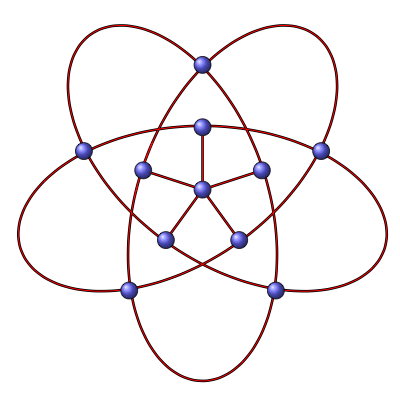
\includegraphics[width=0.75\textwidth]{graph.png}
%\caption{My figure.}
%\label{fig:myfig}
%\end{figure}

\chapter{ Fraud in Context}
\label{sec:context}

\pagebreak

\section{ Interviews from Professionals}

This section will be about what professionals are doing in the fraud field.

\pagebreak

\section{ Research Versus Reality}
\label{sec:rvr}

This section I will compare whatever I find out from professionals to the most modern research on this topic. I assume research will be slightly behind what these professionals are dealing with and how they are solving these problems.

%(As promised in Chapter~\ref{sec:intro}, here it gets interesting.)
\pagebreak


\chapter{Implementing a Fraud Detection System}
\pagebreak

\section{Model}

This section is where I will talk about the overall system I am planning on implementing.

\pagebreak

\section{Experiment}
\pagebreak

\subsection{Hypothesis}
\pagebreak

\subsection{Data}
\pagebreak

\subsection{Methods}

LOTS of Machine Learning incorporated into bigger fraud detection and rule based learning systems! Overall system will be discussed in Model section.
\pagebreak

\subsection{Results}

This section will be full of tables and figures. There will probably also be an appendix with the entire set of experiments run. The most interesting or a subset of the experimental runs will be in a table in this section.
\pagebreak

\subsection{Discussion}

This section will compare my hypothesis to the results, as well as my results to the model I'm basing it off of. I also plan on adding any notes I learn along the way of this implementation.
\pagebreak


\chapter{Further Applications}
\pagebreak

\section{Anomoly Detection}
\pagebreak

\subsection{Cell Phone Fraud}
\pagebreak

\subsection{Biometric Fraud}
\pagebreak

\subsection{Bioinformatics}
\pagebreak

\chapter{Conclusions}
\pagebreak

%\appendix
%\chapter{Chapter 1 of appendix}
%Appendix chapter 1 text goes here

\bibliography{sampleThesis}

\end{document}
